\subsection{Les groupes \texorpdfstring{$\mathbb{Z}_n$}{Zn} et \texorpdfstring{$\mathbb{Z}_n^*$}{Zn*}}

\subsubsection{Définition de \texorpdfstring{$\mathbb{Z}_n$}{Zn}}
\label{sub:def_Z_nZ}

Soit $n$ un entier naturel non nul. 
On définit (dans cette section seulement) la relation $R_n$ sur $\mathbb{Z}$ de la manière suivante : pour tous entiers $a$ et $b$, on a $a \mathop{R_n} b \Leftrightarrow a - b \equiv 0 \, [n]$.

\medskip

\noindent\textbf{Lemme :} $R_n$ est une relation d'équivalence sur $\mathbb{Z}$. 

\medskip

\noindent\textbf{Démonstration :} 
\begin{itemize}[nosep]
    \item Réflexivité : Soit $x$ un élément de $\mathbb{Z}$. 
        On a $x - x = 0$, donc $x - x \equiv 0 \, [n]$, donc $x \mathop{R_n} x$.
    \item Symétrie : Soit $a$ et $b$ deux entiers tels que $a \mathop{R_n} b$.
        Alors, $a - b \equiv 0 \, [n]$.
        Donc (et puisque $-0 = 0$), $b - a \equiv 0 \, [n]$.
        Donc, $b \mathop{R_n} a$.
    \item Transitivité : Soit $a$, $b$ et $c$ trois entiers tels que $a \mathop{R_n} b$ et $b \mathop{R_n} c$.
        Alors, $a - b \equiv 0 \, [n]$ et $b - c \equiv 0 \, [n]$.
        Donc (et puisque $0 + 0 = 0$), $(a - b) + (b - c) \equiv 0 \, [n]$.
        Donc, $a - c \equiv 0 \, [n]$.
        Donc, $a \mathop{R_n} c$.
\end{itemize}

\done

\medskip

Dans cette section et les deux suivantes, pour tout entier $m$, on note $\bar{m}$ la classe d'équivalence de $n$ pour la relation $R_n$.
Notons que chaque classe d'équivalence a un unique représentant dans l'intervalle $[\![0, n-1]\!]$. 
En effet,
\begin{itemize}[nosep]
    \item \emph{Existence :} Soit $x$ une classe d'équivalence et $k$ un de ses éléments.
        Soit $r$ le reste de la division euclidienne de $k$ par $n$.
        Alors, $k - r \equiv 0 \, [n]$, donc $r \in x$, et $r \in [\![0, n-1]\!]$ par définition.
    \item \emph{Unicité :} Soit $k$ et $l$ deux éléments d'une même classe d'équivalence tels que $k \in [\![0, n-1]\!]$ et $k \in [\![0, n-1]\!]$.
        Alors, $0 \leq k \leq n-1$ et $0 \leq l \leq n-1$, donc $1-n \leq k - l \leq n-1$.
        Puisque $k$ et $l$ appartiennent à la même classe d'équivalence, on peut choisir un entier relatif $a$ tel que $k - l = a n$.
        Si $a > 0$, alors $k - l \geq n$, ce qui est impossible.
        Si $a < 0$, alors $k - l \leq -n$, ce qui est impossible.
        Donc, $a = 0$, donc $k = l$.
\end{itemize}

\medskip

\noindent\textbf{Définition :} On note $\mathbb{Z} \divslash (n \mathbb{Z})$, ou plus simplement $\mathbb{Z}_n$\sindex[isy]{$\mathbb{Z}_n$}, l'ensemble des classes d'équivalence de la relation $R_n$.

\medskip

\noindent\textbf{Lemme :} Le cardinal de $\mathbb{Z}_n$ est $n$.

\medskip

\noindent\textbf{Démonstration :}
    Soit $f$ la fonction de $n$ vers $\mathbb{Z}_n$ qui à tout entier naturel $m$ strictement inférieur à $n$ associe $\bar{m}$.
    \begin{itemize}
        \item Soit $a$ et $b$ deux entiers naturels strictement inférieurs à $n$ tels que $f(a) = f(b)$.
            Alors, $\bar{a} = \bar{b}$, donc $b \in \bar{a}$, donc $a \mathop{R_n} b$.
            Donc, $a - b \equiv 0 \, [n]$.
            Donc, $a - b$ est un multiple de $n$.
            Donc, on peut choisir un entier $k$ tel que $a-b = k n$.
            Puisque $-b \leq a-b$ et $a-b \leq a$, on a $-n < a-b$ et $a-b < n$, donc $\abs{a-b} < n$. 
            Donc, $\abs{k} \times n < n$. 
            La seule possibilité est $k = 0$. 
            Donc, $a - b = 0$, et donc $a = b$.
            Cela montre que $f$ est injective.
        \item Soit $y$ un élément de $\mathbb{Z}_n$.
            Par définition d'une classe d'équivalence, $y$ contient au moins un élément $e$.
            Soit $x$ le reste de la division euclidienne de $e$ par $n$.
            Alors, $x$ est un entier naturel strictement inférieur à $n$. 
            En outre, on peut choisir un entier $k$ tel que $x + k \times n = e$.
            On a donc $e - x = k \times n$, donc $e - x = 0$, donc $e \mathop{R_n} x$, donc $\bar{x} = \bar{e}$, et donc $f(x) = y$.
            Cela montre que $f$ est surjective.
    \end{itemize}
    Ainsi, $f$ est une bijection de $n$ vers $\mathbb{Z_n}$.
    Cela montre que $\mathbb{Z}_n$ est de cardinal $n$.

    \done

\medskip

\noindent\textbf{Définition :} On définit les deux lois de composition interne $+$ et $\times$ sur $\mathbb{Z}_n$ de la manière suivante.
    Soit $A$ et $B$ deux éléments de $\mathbb{Z}_n$.
    On pose : $A + B = \overline{a + b}$ et $A \times B = \overline{a \times b}$, où $a$ est un élément de $A$ et $b$ est un élément de $B$ (qui existent par définition d'une classe d'équivalence). 

\medskip

Cette définition requiert que les résultats ne dépendent pas du choix de $a$ et de $b$. 
Montrons que c'est bien le cas. 

\medskip

\noindent\textbf{Lemme :} Dans cette définition, les résultats des opérations $+$ et $\times$ ne dépendent pas du choix des éléments de $A$ et $B$.

\medskip

\noindent\textbf{Démonstration :} Avec les mêmes notations, soit $a$ et $a'$ deux éléments de $A$ et $b$ et $b'$ deux éléments de $B$.
    On veut montrer que $\overline{a' + b'} = \overline{a + b}$ et $\overline{a' \times b'} = \overline{a \times b}$.
    Pour ce faire, il suffit de montrer que $a' + b' \mathop{R_n} a + b$ et $a' \times b' \mathop{R_n} a \times b$.

    Puisque $a$ et $a'$ sont deux éléments de $A$, on a $a \mathop{R_n} a'$, donc $a - a' \equiv 0 \, [n]$.
    De même, puisque $b$ et $b'$ sont deux éléments de $B$, on a $b \mathop{R_n} b'$, donc $b - b' \equiv 0 \, [n]$.
    Donc, $(a - a') + (b + b') \equiv 0 \, [n]$. 
    Donc, $(a + b) - (a' + b') \equiv 0 \, [n]$.
    Donc, $a + b \mathop{R_n} a' + b'$.

    En outre, on peut choisir deux entiers $k$ et $l$ tels que $a - a' = k n$ et $b - b' = l n$.
    Donc, $a b = (a' + k n) (b' + l n) = a' b' + (k + l + k l) n$.
    Donc, $a b - a' b' \equiv 0 \, [n]$.
    Donc, $a b \mathop{R_n} a' b'$.

    \done

\medskip

\noindent\textbf{Lemme :} Le magma $\left( \mathbb{Z}_n, + \right)$ est un group abélien. 
    Ce groupe est parfois noté simplement $\mathbb{Z} \divslash (n \mathbb{Z})$ ou $\mathbb{Z}_n$ quand il n'y a pas de confusion possible.

\medskip

\noindent\textbf{Démonstration :} 
\begin{itemize}[nosep]
    \item L'élément $\bar{0}$ est un élément neutre pour $+$.
        En effet, soit $A$ un élément de $\mathbb{Z}_n$ et $a$ un élément de $A$, on a $\bar{0} + A = \overline{0+a} = \bar{a} = A$ et $A + \bar{0} = \overline{a+0} = \bar{a} = A$.
        Donc, le magma $\left( \mathbb{Z}_n, + \right)$ est unifère.
    \item Soit $A$, $B$ et $C$ trois éléments de $\mathbb{Z}_n$, $a$ un élément de $A$, $b$ un élément de $B$, et $c$ un élément de $C$.
        On a : $A + (B + C) = \bar{a} + \overline{b+c} = \overline{a+(b+c)} = \overline{(a+b)+c} = \overline{a+b} + \bar{c} = (A + B) + C$.
        Donc, la loi de composition interne $\times$ est associative.
        Donc, le magma $\left( \mathbb{Z}_n, + \right)$ est associatif, et donc un monoïde.
    \item Soit $A$ un élément de $\mathbb{Z_n}$. 
        Soit $a$ un élément de $A$.
        Alors, $A + \overline{-a} = \overline{a+(-a)} = \bar{0}$ et $\overline{-a} + A = \overline{-a+a} = \bar{0}$.
        Donc, $\overline{-a}$ est un inverse de $A$ pour $+$.
        Cela montre que $\left( \mathbb{Z}_n, + \right)$ est un groupe.
    \item Soit $A$ et $B$ deux éléments de $\mathbb{Z}_n$, $a$ un élément de $A$, et $b$ un élément de $B$. 
        On a : $A + B = \overline{a+b} = \overline{b+a} = B + A$.
        Donc, la loi de composition interne $+$ est associative.
        Donc, $\left( \mathbb{Z}_n, + \right)$ est un groupe abélien.
\end{itemize}

\done

\medskip

\noindent\textbf{Lemme :} Le triplet $\left( \mathbb{Z}_n, +, \times \right)$ est un anneau commutatif et unifère. 
    L'élément neutre pour $+$ est $\bar{0}$ et l'élément neutre pour $\times$ est $\bar{1}$.

\medskip

\noindent\textbf{Démonstration :} 
\begin{itemize}[nosep]
    \item On a vu que $\left( \mathbb{Z}_n, + \right)$ est un groupe abélien.
    \item Soit $A$, $B$ et $C$ trois éléments de $\mathbb{Z}_n$, $a$ un élément de $A$, $b$ un élément de $B$, et $c$ un élément de $C$.
        On a : $A \times (B + C) = \bar{a} \times \overline{b+c} = \overline{a \times (b+c)} = \overline{(a \times b) + (a \times c)} = \overline{a \times b} + \overline{a \times c} = (A \times B) + (A \times C)$ et $(A+B) \times C  = \overline{a+b} \times \bar{c} = \overline{(a+b) \times c} = \overline{(a \times c) + (b \times c)} = \overline{a \times c} + \overline{b \times c} = (A \times C) + (B \times C)$.
        Donc, $\times$ est distributive sur $+$.
        Donc, $\left( \mathbb{Z}_n, +, \times \right)$ est un anneau.
    \item La classe d'équivalence $\bar{1}$ est un élément neutre pour $\times$. 
        En effet, soit $A$ un élément de $\mathbb{Z}_n$ et $a$ un élément de $A$, on a $A \times \bar{1} = \overline{a \times 1} = \bar{a} = A$ et $\bar{1} \times A = \overline{1 \times a} = \bar{a} = A$.
        Donc, l'anneau $\left( \mathbb{Z}_n, +, \times \right)$ est unifère.
    \item La loi de composition interne $\times$ est commutative.
        En effet, soit $A$ et $B$ deux éléments de $\mathbb{Z}_n$, $a$ un élément de $A$ et $b$ un élément de $B$, on a $A \times B = \overline{a \times b} = \overline{b \times a} = B \times A$.
        Donc, l'anneau $\left( \mathbb{Z}_n, +, \times \right)$ est commutatif.
\end{itemize}

\done

\medskip

À titre d'exemple, les tables d'addition et de multiplication dans $(\mathbb{Z}_10, +, \times)$ sont données table~\ref{tab:Z10}. 
Les figures~\ref{fig:ZqZ_circle} et~\ref{fig:ZqZ_circle_add} montrent une représentation géométrique de $\mathbb{Z}_n$ pour quelques valeurs de $n$ ainsi que de l'addition sur $(\mathbb{Z}_n, +)$.

\begin{table}
    \newcolumntype{?}{!{\vrule width 1pt}}
    \aboverulesep = 0mm 
    \belowrulesep = 0mm
    \centering
    \begin{tabular}{ c ? c | c | c | c | c | c | c | c | c | c |}
        + & 0 & 1 & 2 & 3 & 4 & 5 & 6 & 7 & 8 & 9 \\
        \midrule[1pt]
        0 & 0 & 1 & 2 & 3 & 4 & 5 & 6 & 7 & 8 & 9 \\
        \hline
        1 & 1 & 2 & 3 & 4 & 5 & 6 & 7 & 8 & 9 & 0 \\
        \hline
        2 & 2 & 3 & 4 & 5 & 6 & 7 & 8 & 9 & 0 & 1 \\
        \hline
        3 & 3 & 4 & 5 & 6 & 7 & 8 & 9 & 0 & 1 & 2 \\
        \hline
        4 & 4 & 5 & 6 & 7 & 8 & 9 & 0 & 1 & 2 & 3 \\
        \hline
        5 & 5 & 6 & 7 & 8 & 9 & 0 & 1 & 2 & 3 & 4 \\
        \hline
        6 & 6 & 7 & 8 & 9 & 0 & 1 & 2 & 3 & 4 & 5 \\
        \hline
        7 & 7 & 8 & 9 & 0 & 1 & 2 & 3 & 4 & 5 & 6 \\
        \hline
        8 & 8 & 9 & 0 & 1 & 2 & 3 & 4 & 5 & 6 & 7 \\
        \hline
        9 & 9 & 0 & 1 & 2 & 3 & 4 & 5 & 6 & 7 & 8 \\
        \hline
    \end{tabular}
    \hspace*{1.5em}
    \begin{tabular}{ c ? c | c | c | c | c | c | c | c | c | c |}
        × & 0 & 1 & 2 & 3 & 4 & 5 & 6 & 7 & 8 & 9 \\
        \midrule[1pt]
        0 & 0 & 0 & 0 & 0 & 0 & 0 & 0 & 0 & 0 & 0 \\
        \hline
        1 & 0 & 1 & 2 & 3 & 4 & 5 & 6 & 7 & 8 & 9 \\
        \hline
        2 & 0 & 2 & 4 & 6 & 8 & 0 & 2 & 4 & 6 & 8 \\
        \hline
        3 & 0 & 3 & 6 & 9 & 2 & 5 & 8 & 1 & 4 & 7 \\
        \hline
        4 & 0 & 4 & 8 & 2 & 6 & 0 & 4 & 8 & 2 & 6 \\
        \hline
        5 & 0 & 5 & 0 & 5 & 0 & 5 & 0 & 5 & 0 & 5 \\
        \hline
        6 & 0 & 6 & 2 & 8 & 4 & 0 & 6 & 2 & 8 & 4 \\
        \hline
        7 & 0 & 7 & 4 & 1 & 8 & 5 & 2 & 9 & 6 & 3 \\
        \hline
        8 & 0 & 8 & 6 & 4 & 2 & 0 & 8 & 6 & 4 & 2 \\
        \hline
        9 & 0 & 9 & 8 & 7 & 6 & 5 & 4 & 3 & 2 & 1 \\
        \hline
    \end{tabular}
    \caption{Tables d'addition (gauche) et de multiplication (droite) dans $\mathbb{Z}_{10}$. 
             Chaque élément de $\mathbb{Z}_{10}$ est représenté par son unique élément dans $[\![0, 9]\!]$.}
    \label{tab:Z10}
\end{table}

\begin{figure}
    \centering
    \def\maxN{8}
    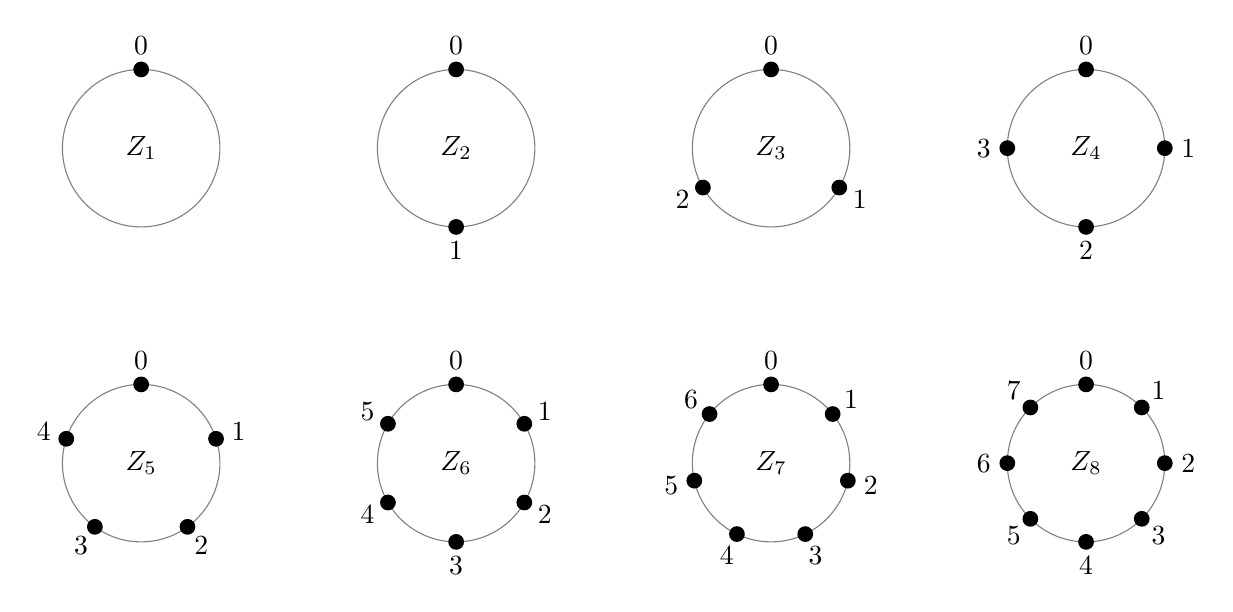
\begin{tikzpicture}
        \def\figHSpace{4}
        \def\figVSpace{4}
        \def\figRadius{1}
        \def\figRadiusL{1.3}
        \def\figPointSize{0.1}
        \def\nCirclesPerLine{4}
        \foreach[evaluate=\i as \im using {Mod(\i-1, \nCirclesPerLine)}] \i in {1, ..., \maxN} {
            \pgfmathsetmacro\line{(\i - 1 - \im) / \nCirclesPerLine}
            \node at (\im*\figHSpace, -\line*\figVSpace) {$\mathbb{Z}_\i$};
            \draw[gray] (\im*\figHSpace, -\line*\figVSpace) circle(\figRadius);
            \foreach[evaluate=\j as \k using int(\j-1)] \j in {1, ..., \i} {
                \fill[black] ({\im * \figHSpace + \figRadius * sin(360*\k/\i)}, 
                              {\figRadius * cos(360*\k/\i) - \line * \figVSpace}) circle(\figPointSize);
                \node at ({\im * \figHSpace + \figRadiusL * sin(360*\k/\i)}, 
                          {\figRadiusL * cos(360*\k/\i) - \line * \figVSpace}) {$\k$};
            }
        }
    \end{tikzpicture}
    \caption{Illustration des groupes $\mathbb{Z}_n$ pour $n$ décrivant $[\![1, \maxN]\!]$. 
        Pour chaque valeur de $n$, $\mathbb{Z}_n$ peut être représenté par $n$ points équidistants sur un cercle. 
        (Ici, ses éléments sont représentés par leur unique représentant dans $[\![1, n]\!]$.) 
        Pour tout élément $\bar{m}$ de $\mathbb{Z}_n$, la fonction $x \mapsto x + \bar{m}$ est alors équivalente à une rotation d'une fraction $m \divslash n$ de cercle (soit $2 \pi m \divslash n$ radians, ici dans le sens horaire), où $m$ est un représentant de $\bar{m}$ (voir figure~\ref{fig:ZqZ_circle_add}).
        }
    \label{fig:ZqZ_circle}
\end{figure}

\begin{figure}
    \centering
    \def\valN{6}
    \begin{tikzpicture}
        \def\figHSpace{5}
        \def\figVSpace{4}
        \def\figRadius{1}
        \def\figRadiusL{1.3}
        \def\figRadiusLb{1.8}
        \def\figPointSize{0.1}
        \def\nCirclesPerLine{3}
        \foreach[evaluate=\i as \im using {int(Mod(\i-1, \nCirclesPerLine))}] \i in {1, ..., \valN} {
            \pgfmathsetmacro\line{(\i - 1 - \im) / \nCirclesPerLine}
            \pgfmathsetmacro\ima{int(Mod(\i - 1, \valN))}
            \node at (\im*\figHSpace, -\line*\figVSpace - \figRadiusLb) {$ + \ima$};
            \draw[gray] (\im*\figHSpace, -\line*\figVSpace) circle(\figRadius);
            \foreach[evaluate=\j as \k using int(\j-1)] \j in {1, ..., \valN} {
                \fill[black] ({\im * \figHSpace + \figRadius * sin(360*\k/\valN)}, 
                              {\figRadius * cos(360*\k/\valN) - \line * \figVSpace}) circle(\figPointSize);
                \node at ({\im * \figHSpace + \figRadiusL * sin(360*\k/\valN)}, 
                          {\figRadiusL * cos(360*\k/\valN) - \line * \figVSpace}) {$\k$};
                \pgfmathparse{\i}
                \ifnum\pgfmathresult>1
                    \draw[-Latex] ({\im * \figHSpace + \figRadius * sin(360*\k/\valN)}, 
                                   {\figRadius * cos(360*\k/\valN) - \line * \figVSpace}) 
                        -- ({\im * \figHSpace + \figRadius * sin(360*(\k+\i-1)/\valN)}, 
                            {\figRadius * cos(360*(\k+\i-1)/\valN) - \line * \figVSpace});
                \fi
            }
        }
    \end{tikzpicture}
    \caption{Illustration de l'addition sur $\mathbb{Z}_\valN$, sous la représentation de la figure~\ref{fig:ZqZ_circle}. 
        }
    \label{fig:ZqZ_circle_add}
\end{figure}

\medskip

\noindent\textbf{Lemme :} Si $n$ est un nombre premier, le triplet $\left( \mathbb{Z}_n, +, \times \right)$ est un corps. 

\medskip

\noindent\textbf{Démonstration :} 
\begin{itemize}[nosep]
    \item L'ensemble $\mathbb{Z}_n$ est de cardinal $n$. 
        Si $n$ est premier, $n > 1$, donc l'anneau $\left( \mathbb{Z}_n, +, \times \right)$ n peut être nul.
    \item Soit $A$ un élément de $\mathbb{Z}_n$ tel que $A \neq \bar{0}$.
        Soit $a$ un éllément de $A$. 
        Alors, $a$ n'est pas un multiple de $n$ (sans quoi on aurait $a \equiv 0 \, [n]$, et donc $A = \bar{0}$).
        Donc, d'après le petit théorème de Fermat, $a^{n-1} \equiv 1 \, [n]$. 
        Puisque $n$ est premier, $n \geq 2$, donc $n-2$ est un entier naturel et, d'après l'équation précédente, $a \times a^{n-2} \equiv 1 \, [n]$. 
        Donc, $a \times a^{n-2} \mathop{R_n} 1$.
        Donc, $\overline{a \times a^{n-2}} = \bar{1}$.
        Donc, $A \times \overline{a^{n-2}} = \bar{1}$.
        Puisque $\times$ est commutative, cela implique également $\overline{a^{n-2}} \times A = \bar{1}$.
        Donc, $\overline{a^{n-2}}$ est un inverse de $A$ pour $\times$.
\end{itemize}

\done

\medskip

\noindent\textbf{Lemme :} Si $n$ n'est pas un nombre premier, le triplet $\left( \mathbb{Z}_n, +, \times \right)$ n'est pas un corps. 

\medskip

\noindent\textbf{Démonstration :} 
    Si $n = 1$, alors $\mathbb{Z}_n$ ne contient qu'un seul élément, donc l'anneau $\left(\mathbb{Z}_n, +, \times \right)$ est nul et n'est donc pas un corps.

    Sinon, et si $n$ n'est pas premiers, on peut choisir deux entiers naturels $p$ et $q$ tels que $p < n$, $q < n$ et $p \times q = n$ (par example, on peut prendre pour $p$ un diviseur premier de $n$ et $q = n / p$).
    On a alors $\bar{p} \neq \bar{0}$, $\bar{q} \neq \bar{0}$, et $\bar{p} \times \bar{q} = \bar{0}$, ce qui (puisque $\bar{0}$ est l'élément neutre de $+$) serait impossible si $\left(\mathbb{Z}_n, +, \times \right)$ était un corps. 

    \done

\medskip

\noindent\textbf{Remarque :} La dernière partie de la démonstration montre que, si $n$ est strictement supérieur à $1$ et n'est pas un nombre premier, alors $\times$ ne définit pas une loi de composition interne sur $\mathbb{Z}_n \setminus \lbrace \bar{0} \rbrace$.

\subsubsection{Définition de \texorpdfstring{$\mathbb{Z}_n^*$}{Zn*}}

Soit $n$ un entier naturel non nul. 
On définit l'enemble $\left( \mathbb{Z} \divslash (n \mathbb{Z}) \right)^*$, aussi noté $\mathbb{Z}_n^*$, comme le sous-ensemble de $\mathbb{Z}_n$ défini comme suit : pour tout élément $z$ de $\mathbb{Z}_n$, soit $x$ un représentant de $z$, alors $z \in \mathbb{Z}_n^*$ si et seulement si $\mathrm{pgcd}(\abs{x}, n) = 1$.

Montrons que cette définition ne dépend pas du représentant choisi. 
Soit $k$ et $l$ deux représentants d'une même classe d'équivalence. 
On suppose que $\mathrm{pgcd}(\abs{k}, n) = 1$.
Soit $d$ un diviseur commun à $\abs{l}$ (et donc à $l$) et à $n$. 
Puisque $k$ et $l$ sont dans la même classe d'équivalence, on peut choisir un entier relatif $m$ tel que $k = n + l m$.
Donc, $d$ est un diviseur de $k$, et donc de $\abs{k}$. 
Donc, $d$ est un diviseur commun à $k$ et à $n$. 
Donc, $d$ ne peut qu'être égal à $1$.
On en déduit que $\mathrm{pgcd}(\abs{l}, n) = 1$.

Soit $p$ un nombre premier. 
Alors $\left( \mathbb{Z} \divslash (p \mathbb{Z}) \right)^*$, aussi noté $\mathbb{Z}_p^*$, satisfait : $\mathbb{Z}_p^* = \mathbb{Z}_p \setminus \lbrace \bar{0} \rbrace$.
Puisque $\left(\mathbb{Z}_p, +, \times \right)$ est un corps et puisque $\bar{0}$ est l'élément neutre de la loi de composition interne $+$, $\left( \mathbb{Z}_p^*, \times \right)$ (où $\times$ désigne la restriction de la loi de composition interne définie ci-dessus à $\mathbb{Z}_p^*$) est un groupe abélien, parfois noté simplement $\left( \mathbb{Z} \divslash (p \mathbb{Z}) \right)^*$ ou $\mathbb{Z}_p^*$ quand il n'y a pas de confusion possible.

\medskip

\noindent
\textbf{Lemme :} Soit $n$ un entier naturel non nul. Alors $\left( \mathbb{Z}_n, \times \right)$ est un groupe abélien, d'élément neutre $\bar{1}$.

\medskip

\noindent
\textbf{Démonstration :} Notons que $\bar{1} \in \mathbb{Z}_n^*$ puisque le plus grand diviseur de $1$ est $1$ lui-même, donc $\mathrm{pgcd}(1, n) = 1$. 
\begin{itemize}[nosep]
    \item \emph{L'opération $\times$ est une loi de composition interne :} Soit $\bar{a}$ et $\bar{b}$ deux éléments de $\mathbb{Z}$, $a$ un représentant de $\bar{a}$ et $b$ un représentant de $\bar{b}$.
        Alors, $\abs{a}$ et $\abs{b}$ sont chacun premiers avec $n$.
        Donc, $\abs{ab}$ est premier avec $n$.
        Donc, $\overline{ab} \in \mathbb{Z}_n^*$.
        Donc, $\bar{a} \times \bar{b} \in \mathbb{Z}_n^*$.
    \item \emph{Associativité, commutativité et $\bar{1}$ comme élément neutre :} Ces propriétés découlent directement du fait que $(\mathbb{Z}_n, +, \times)$ est un anneau unifère d'élément neutre $\bar{1}$ pour l'opération $\times$. 
    \item \emph{Existence d'un inverse pour tout élément de $\mathbb{Z}_n^*$ :}
        Soit $\bar{a}$ un élément de $\mathbb{Z}_n$ et $a$ son unique représentant dans $[\![0, n-1]\!]$. 
        Soit $f$ la fonction de $\mathbb{Z}_n$ vers lui-même définie par : pour tout élément $\bar{b}$ de $\mathbb{Z}_n$, $f(\bar{b}) = \bar{a} \times \bar{b}$.
        Soit $\bar{b}$ et $\bar{c}$ deux éléments de $\mathbb{Z}_n$, $b$ et $c$ leurs représentants respectifs dans $[\![0, n-1]\!]$, et supposons que $f(\bar{b}) = f(\bar{c})$. 
        Alors, $\bar{a} \times \bar{b} = \bar{a} \times \bar{c}$. Donc, $\overline{a \times b} = \overline{a \times c}$.
        Donc, $a \times b - a \times c \equiv 0 \, [n]$.
        Donc, $a \times (b - c) \equiv 0 \, [n]$.
        Donc, $a \times \abs{b - c} \equiv 0 \, [n]$. (En effet, $a \times \abs{b - c} = a \times (b - c)$ si $b \geq c$ ou $a \times \abs{b - c} = -(a \times (b - c))$ si $b < c$.)
        Puisque $a$ est premier avec $n$, on en déduit que $\abs{b - c}$ est un multiple de $n$.
        Puisque $b-c$ est dans $[\![-(n-1), n-1]\!]$, $\abs{b-c} < n$. 
        Le seul multiple de $n$ satisfaisant cette propriété est $0$.
        (En effet, si $a$ est un entier relatif, alors $\abs{a n} = \abs{a} n$, donc $\abs{a n} \geq n$ sauf si $a = 0$.)
        Donc, $b = c$, et donc $\bar{b} = \bar{c}$.
        Cela montre que $f$ est injective. 
        Puisque $\mathbb{Z}_n$ est fini (de cardinal $n$) et $\mathbb{Z}_n^*$ est un sous-ensemble de $\mathbb{Z}_n$, $\mathbb{Z}_n^*$ est également fini. 
        Donc, $f$ est bijective. 
        Donc, on peut choisir un élément $x$ de $\mathbb{Z}_n^*$ tel que $\bar{a} \times x = \bar{1}$. 
        Puisque $\times$ est commutative, on en déduit que $x$ est un inverse de $\bar{a}$.
\end{itemize}

\done

\medskip

À titre d'exemple, les tables de multiplication dans $(\mathbb{Z}_5^*, \times)$ et $(\mathbb{Z}_{10}^*, \times)$ sont données table~\ref{tab:Z10star}.
Ces tables motrent que la fonction $f: \mathbb{Z}_5^* \to \mathbb{Z}_{10}^*$ définie par $f(\bar{1}) = \bar{1}$, $f(\bar{2}) = \bar{3}$, $f(\bar{3}) = \bar{7}$ et $f(\bar{4}) = \bar{9}$ est un isomorphisme de groupes (de $(\mathbb{Z}_5^*, \times)$ vers $(\mathbb{Z}_{10}^*, \times)$).

\begin{table}
    \newcolumntype{?}{!{\vrule width 1pt}}
    \aboverulesep = 0mm 
    \belowrulesep = 0mm
    \centering
    \begin{tabular}{ c ? c | c | c | c |}
        × & 1 & 2 & 3 & 4 \\
        \midrule[1pt]
        1 & 1 & 2 & 3 & 4 \\
        \hline
        2 & 2 & 4 & 1 & 3 \\
        \hline
        3 & 3 & 1 & 4 & 2 \\
        \hline
        4 & 4 & 3 & 2 & 1 \\
        \hline
    \end{tabular}
    \hspace*{5em}
    \begin{tabular}{ c ? c | c | c | c |}
        × & 1 & 3 & 7 & 9 \\
        \midrule[1pt]
        1 & 1 & 3 & 7 & 9 \\
        \hline
        3 & 3 & 9 & 1 & 7 \\
        \hline
        7 & 7 & 1 & 9 & 3 \\
        \hline
        9 & 9 & 7 & 3 & 1 \\
        \hline
    \end{tabular}
    \caption{Tables de multiplication dans $\mathbb{Z}_5^*$ (gauche) et $\mathbb{Z}_{10}^*$ (droite). 
             Chaque élément de $\mathbb{Z}_n^*$ est repréenté par son unique élément dans $[\![0, n-1]\!]$ pour $n \in \lbrace 5, 10 \rbrace$.}
    \label{tab:Z10star}
\end{table}

\subsubsection{Cyclicité de \texorpdfstring{$\left( \mathbb{Z} \divslash (p \mathbb{Z}) \right)^*$}{(Z / p Z)*} pour \texorpdfstring{$p$}{p} premier}
\label{subsubsec:cyclicity_Z_pZ}

\textit{À écrire}
